
\begin{frame}
  \frametitle{Learning Curves : Linear Model}
  \begin{figure}
    \begin{minipage}{0.65\textwidth}
      \centering
      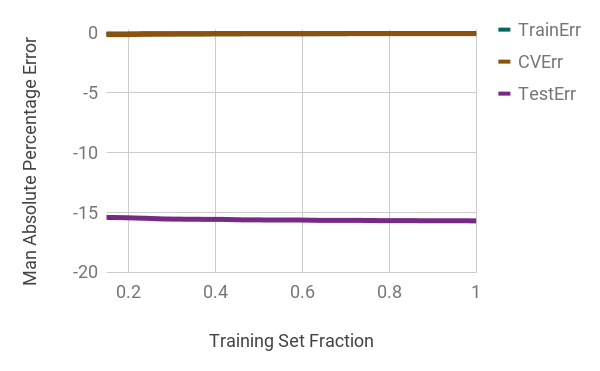
\includegraphics[width=\linewidth]{./figures/rr-learn.png}
    \end{minipage}%
    \begin{minipage}{0.35\textwidth}
      \centering
      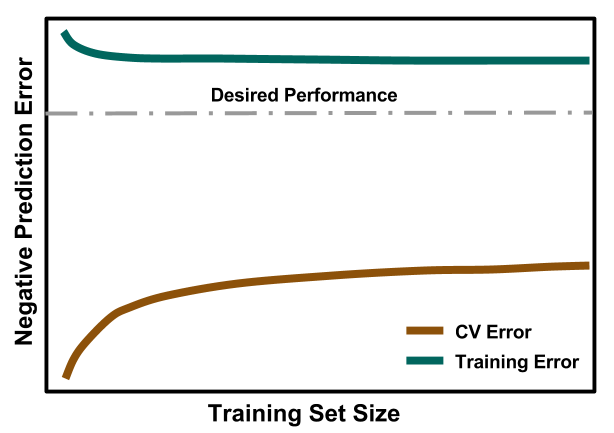
\includegraphics[width=\linewidth]{./figures/NegLearningCurve-variance.png}
    \end{minipage}
    \caption{Learning curve and comparison schematic for ridge regression; $\alpha=1.0$}
  \end{figure}
\end{frame}

\begin{frame}
  \frametitle{Learning Curves : \textit{k}-Nearest Neighbors}
  \begin{figure}
    \begin{minipage}{0.65\textwidth}
      \centering
      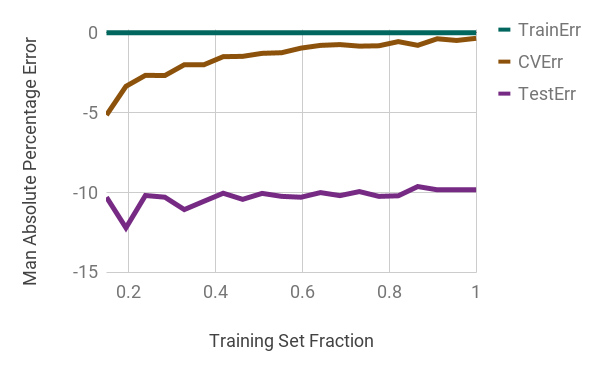
\includegraphics[width=\linewidth]{./figures/nn-learn.png}
    \end{minipage}%
    \begin{minipage}{0.35\textwidth}
      \centering
      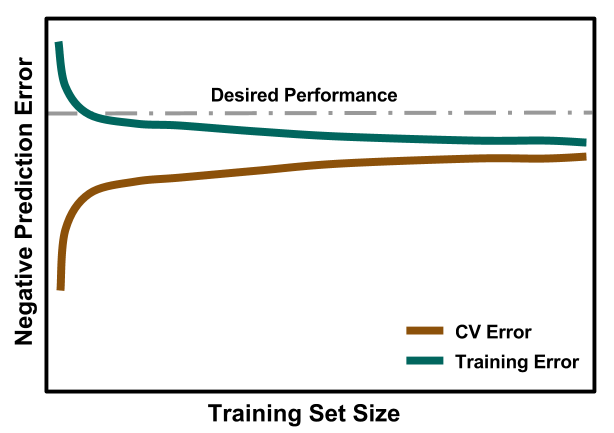
\includegraphics[width=\linewidth]{./figures/NegLearningCurve-ideal.png}
      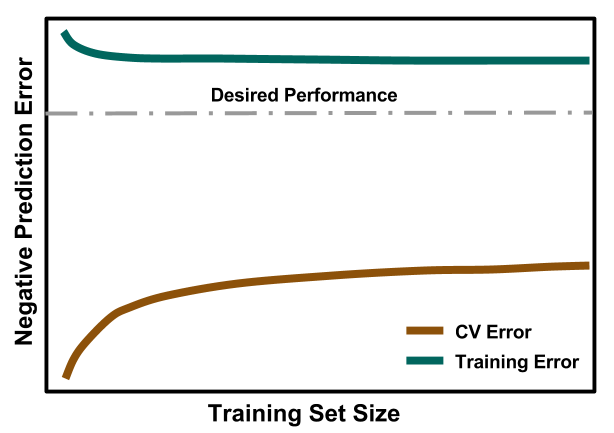
\includegraphics[width=\linewidth]{./figures/NegLearningCurve-variance.png}
    \end{minipage}
    \caption{Learning curve and comparison schematic for \textit{k}-NN regression; $k=1$}
  \end{figure}
\end{frame}

\begin{frame}
  \frametitle{Learning Curves: Support Vectors}
  \begin{figure}
    \begin{minipage}{0.65\textwidth}
      \centering
      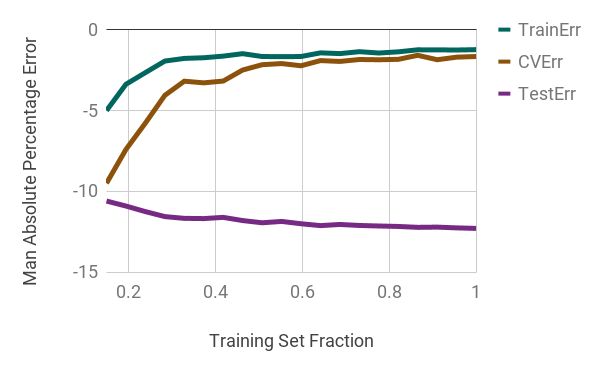
\includegraphics[width=\linewidth]{./figures/svr-learn.png}
    \end{minipage}%
    \begin{minipage}{0.35\textwidth}
      \centering
      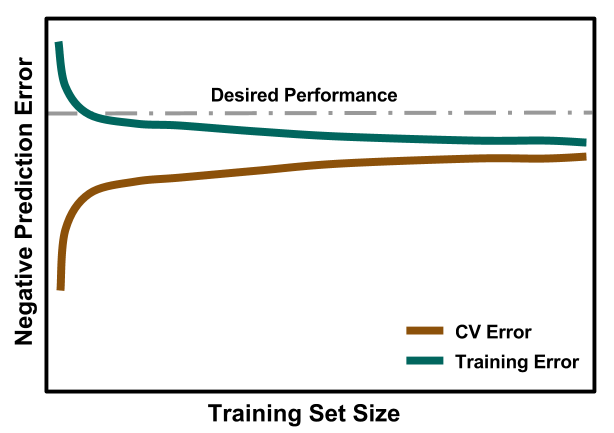
\includegraphics[width=\linewidth]{./figures/NegLearningCurve-ideal.png}
      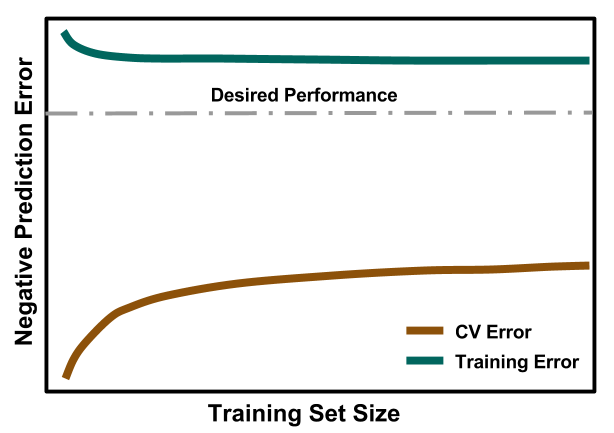
\includegraphics[width=\linewidth]{./figures/NegLearningCurve-variance.png}
    \end{minipage}
    \caption{Learning curve and comparison schematic for SVR; $\gamma=10^{-3}$ and $C=10^3$}
  \end{figure}
\end{frame}


\begin{frame}
  \frametitle{Validation Curves : Linear Model}
  \begin{figure}
    \begin{minipage}{0.65\textwidth}
      \centering
      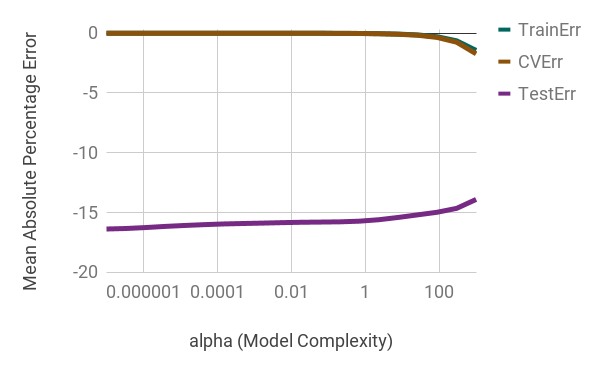
\includegraphics[width=\linewidth]{./figures/rr-valid.png}
    \end{minipage}%
    \begin{minipage}{0.4\textwidth}
      \centering
      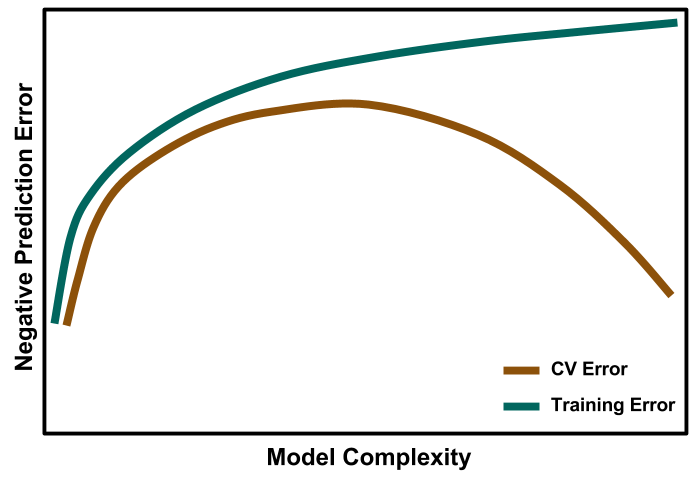
\includegraphics[width=\linewidth]{./figures/NegValidCurve.png}
    \end{minipage}
    \caption{Validation curve and comparison schematic for ridge regression; $Training Set Size=2313$}
  \end{figure}
\end{frame}

\begin{frame}
  \frametitle{Validation Curves : \textit{k}-Nearest Neighbors}
  \begin{figure}
    \begin{minipage}{0.65\textwidth}
      \centering
      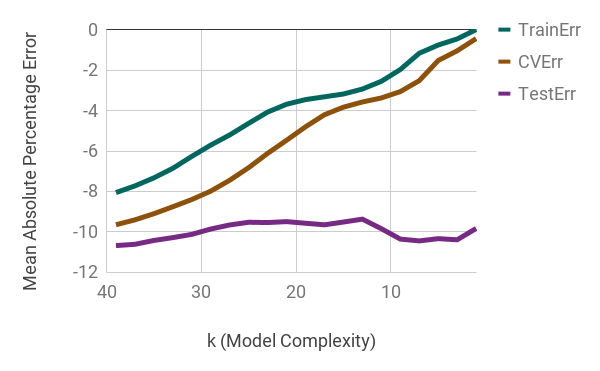
\includegraphics[width=\linewidth]{./figures/nn-valid.png}
    \end{minipage}%
    \begin{minipage}{0.4\textwidth}
      \centering
      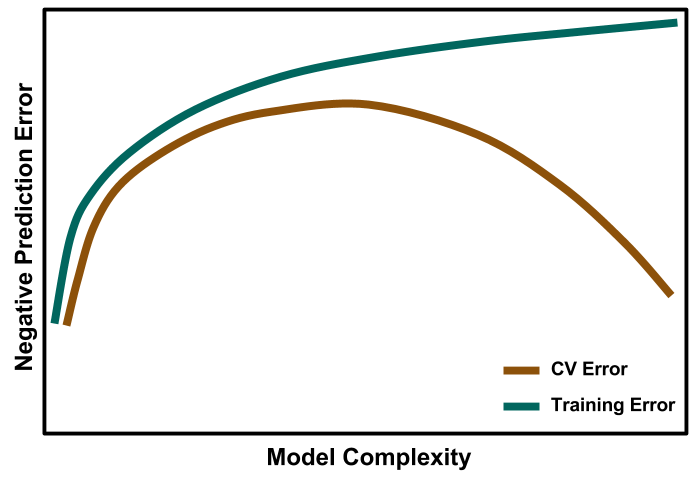
\includegraphics[width=\linewidth]{./figures/NegValidCurve.png}
    \end{minipage}
    \caption{Validation curve and comparison schematic for \textit{k}-NN regression; $Training Set Size=2313$}
  \end{figure}
\end{frame}

\begin{frame}
  \frametitle{Validation Curves : Support Vectors}
  \begin{figure}
    \begin{minipage}{0.65\textwidth}
      \centering
      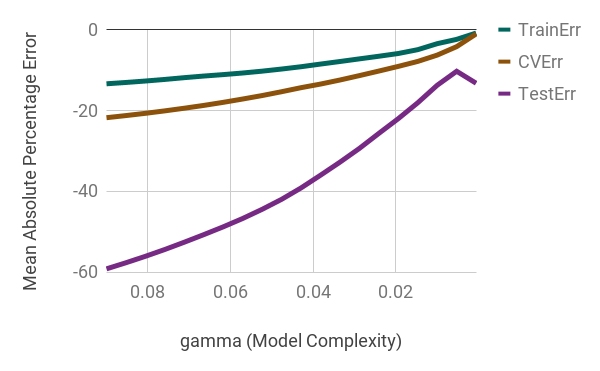
\includegraphics[width=\linewidth]{./figures/svr-valid.png}
    \end{minipage}%
    \begin{minipage}{0.4\textwidth}
      \centering
      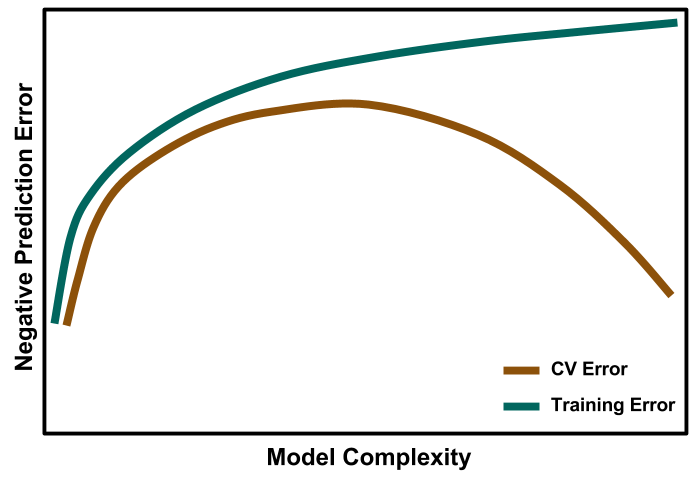
\includegraphics[width=\linewidth]{./figures/NegValidCurve.png}
    \end{minipage}
    \caption{Validation curve and comparison schematic for SVR; $Training Set Size=2313$ and $C=10^3$}
  \end{figure}
  \footnotesize
  Note: Default $\gamma$ would be $~\frac{1}{2000}=0.0005$
\end{frame}

